    \raggedcolumns % блокировка растягивания строк по высоте в следущей колонке
    
    \begin{multicols}{2} % деление на две коллонки
        \noindent \textbf{\LARGE Задачи вступительной контрольной работы в ВЗМШ в 1977 году} \\
        
        \setlist[enumerate,1]{label=\textbf{\arabic* }} % Собственный стиль нумерации (жирный без точек с отступом)
        \begin{enumerate}[itemsep=0pt, wide=0pt, itemindent=3em] % параметры для удаления оступа всего стобца и добавления отступа, как в абзацах
            \item В равенстве двух дробей, числители и знаменатели которых двухзначные числа, цифры заменены буквами одинаковые --- одинаковыми, разные --- разными
            \[\frac{\textit{КУ}}{\textit{РЕ}} = \frac{\textit{КА}}{\textit{КУ}}\]
            \hspace* {3mm} Какую цифру означает каждая из букв (достаточно привести все возможные ответы)?\setlength{\parindent}{1.5em}
            \item Дан прямоугольник \textit{ABCD} Найдите множество точек \textit{M}, для которых
            \[|\textit{MA}|+|\textit{MB}| = |\textit{MC}| + |\textit{MD}|\]
            \item Дополните табличку $4\times4$ (см. рисунок) буквами В, З, М, Ш, объединение их рамками четырех типов (квадрат, ромб, круг, треугольник) и раскрасьте их в четыре цвета так, чтобы выполнялись следующие условия 1) в каждой строчке и в каждом столбце должны встречаться все буквы, цвета и типы рамок, 2) каждая буква должна быть раскрашена по разу каждым цветом, 3) рамка каждого типа должна содержать каждую букву и каждый цвет (Достаточно нарисовать требуемую картинку)
            \item В прямоугольном треугольнике \textit{a} и \textit{b} --- длины его катетов, \textit{c} --- длина гипотенузы, \textit{h} --- длина высоты, опущенной на гипотенузу. Докажите, что $\textit{c} + \textit{h}$ больше $\textit{a} - \textit{b}$
            \item Найдите все решения системы уравнений
            \[
            \begin{cases}
                x^2 = y + z,\\
                y^2 = z + x,\\
                z^2 = x^2 + y^2
            \end{cases}
            \]
            \item Даны две непересекающиеся окружности. Существует ли вне окружностей такая точка, что всякая прямая, проходящая через неё пересекает хотя бы одну из окружностей?\\
            \begin{center}
                \vspace{-\baselineskip}
                \begin{tabular}{|c|c|c|c|}
                    \hline
                     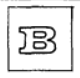
\includegraphics[width=1.5cm,height=1.5cm]{imgs/fig1.png} & 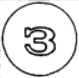
\includegraphics[width=1.5cm,height=1.5cm]{imgs/fig2.png} & 
\includegraphics[width=1.5cm,height=1.5cm]{imgs/fig3.png} & 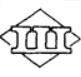
\includegraphics[width=1.5cm,height=1.5cm]{imgs/fig4.png} \\ \hline
                     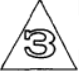
\includegraphics[width=1.5cm,height=1.5cm]{imgs/fig5.png} & & & \\ \hline
                     
\includegraphics[width=1.5cm,height=1.5cm]{imgs/fig6.png} & & & \\ \hline
                     
\includegraphics[width=1.5cm,height=1.5cm]{imgs/fig7.png} & & & \\ \hline
                \end{tabular}
            \end{center}
            \item Автомобиль и велосипедист выехали одновременно из \textit{A} и \textit{B}. Проехав треть пути, велосипедист остановился и тронулся лишь тогда, когда автомобилю оставалась лишь треть пути до \textit{B}. Автомобиль, доехав до \textit{B}, без остановки поехал обратно в \textit{A}. Кто приедет раньше: автомобиль в \textit{A} или велосипедист в \textit{B}?
            \item Известно, что числа 2077 и 100 при делении на натуральное число \textit{a} дают одинаковые остатки. Найдите число \textit{a}
            \item Большой прямоугольник разбит на клетки $1\textit{ см}\times1\textit{ см}$. Внутри каждой клетки написано число. Известно, что сумма всех чисел в каждой горизонтальной строчке равна 1, а в каждом вертикальном столбце --- равна 2. Может ли площадь прямоугольника равняться 1976 $\textit{см}^2$?
            \item Несколько ящиков весят вместе 10 тонн, причем каждый из них весит не больше одной тонны. Какое наименьшее количество трехтонок заведомо достаточно, чтобы увезти этот груз
            \begin{flushright}
                \vspace{-\baselineskip} % flushright добавляет отступ. Убираем его отрицательным отступом
                \textit{Ж. Раббот}
            \end{flushright}
        \end{enumerate}
         
    \end{multicols}
    \begin{center}
        \textbf{\LARGE Заочная физико-техническая школа}    
    \end{center}
    Заочная физико-техническая школа (ЗФТШ) при Московском ордена Трудового Красного Знамени физико-техническом институте проводит набор учащихся восьмилетних и средних школ, расположенных на территории РСФСР, в 8-й, 9-й и 10-й классы на 1977/78 учебный год\\
    \indent Форма обучения в нашей школе отличается от привычной для ребят работы с учителем на уроках. Заочное обучение прививает навыки самостоятельности, учит работать с дополнительной литературой, конспективно излагать свои мысли\\
    \indent За 10 лет работы ЗФТШ дала хорошие дополнительные знания по физике и математике своим выпускникам, многие из которых стали студентами ведущих вузов нашей страны\\
    \indent Цель нашей школы --- помочь ученикам в самостоятельных занятиях по физике и математике. Вот почему при приеме в ЗФТШ предпочтение отдается учащимся, проживающим в сельской местности и в рабочих поселках, где помощь нашей школы особенно нужна\\
    \indent В ЗФТШ принимаются и физико-технические кружки, которые могут быть организованы на месте по инициативе двух преподавателей --- физики и математики. Руководители кружка набирают и зачисляют в них учащихся, успешно выполнивших вступительное задание ЗФТШ. Кружок принимается в ЗФТШ, если директор школы сообщит в ЗФТШ фамилии руководителей кружка и поименный список членов кружка по классам (с указанием итоговых оценок за вступительное задание)
    \begin{flushright}
        \vspace{-\baselineskip}
        \textbf{53}
    \end{flushright}
\end{document}
